\section{Evaluation}

\subsection{Configuration}

We conducted the extensive experiments to evaluate the performance of the methods proposed in this work. In the experiments, we use four nodes as the workers and one node as the master. Each node has two eight-core Xeon-2670 CPUs and 64GB memory. The file system is mounted on a SAS disk, running the RedHat Enterprise Linux 5 (kernel 2.6.18). The JDK version is 1.7.0 for Spark 1.6 and Spark Job Server 0.6.2. We record not only the execution time of each application, but also the detailed runtime situations.

\begin{comment}
\begin{table}[!t]
\small
\centering
\caption{Function APIs in each Application}
\begin{tabular}{ c | c | c | c }

\hline
\textbf{App} & \textbf{Stages} & \textbf{Function API(s)} & \textbf{Cache} \\
\hline
SQ & 1 & \textit{filter} & No \\
\hline
AQ & 2 & \textit{flatMap} \& \textit{reduceByKey} & No \\
\hline
Sort & 3 & \textit{distinct} \& \textit{sortByKey} & No \\
\hline
PR & N & \textit{groupByKey} \& \textit{map} \& \textit{reduceByKey} & Yes \\
\hline

\hline
\end{tabular}
%\vspace{1mm} 
\vspace{-4mm}
\label{table:app}
\end{table} 
\end{comment}

%We choose four typical benchmark applications in Spark to evaluate the performance: Grep, Sort, WordCount(WC) and PangeRank(PR). Grep has only one stage: it filters the records that do not satisfy the conditions. WC has two stages: it counts the number of each key in the input file. Sort has three stages: it sorts all records by key in the input file. While PR is a typical iterative computations, one of its most important features is that it will cache the data in memory.
We choose four applications to evaluate the performance: Scan Query (SQ) and Aggregation Query (AQ) which are exploratory SQL queries in ~\cite{www:benchmark}, Sort and  PageRank(PR) which are typical benchmark applications in Spark. For each query, a semantic-identical hand-written Spark program are used for general cases. PR is a typical iterative computations, one of its most important features is that it will cache the data in memory. Another important features is that each iteration of PR is similar to the Join Query in SQL queries.
%We choose these four benchmarks because these applications contain different function APIs, as shown in Table~\ref{table:app}. 
For Sort and AQ, the datasets are produced by HiBench Random Writer with 1B unique key numbers. The sizes of the input datasets for Sort and AQ are 30GB and 50GB, respectively. For SQ and PR, we use the real graphs, webbase-2001 (30GB)~\cite{boldi:webgraph}, to evaluate the performance of MURS. The key-value pairs of each record in all input dataset have the similar size. We use the heap size to evaluate different memory pressure. The garbage collection time is used to measure the memory pressure. These applications are grouped to evaluate different scenes and submitted to the Spark Job Server together.

\subsection{Memory pressure without caching}

Most current data processing systems are designed based on MapReduce. But only a part of them provide the in-memory computing model that caches the data in memory to speed up the system. Thus, we first evaluate these applications without caching the data in memory, which represents the common frameworks that work with the key-value pairs, such as Hadoop and Hive.

We choose three applications: Sort, AQ, and SQ. These applications do not perform the caching operations. Each application has similar implementation in MapReduce. SQ reads the data from the disk and filters these records which satisfy the given conditions. Most data objects are temporary. The shuffle buffers in Sort and AQ contain the data objects with long lifetime. Thus the tasks in Sort and AQ are the light to heavy tasks in MURS. The results of each submission are shown in Figure~\ref{fig:pressurewithoutcache}. The best improvement achieved by MURS is 1.8x to 2.9x compared to Spark in each evaluation. The reduction of the garbage collection contributes most to the improvement.

\begin{figure*}[!t]
\centering
\subfigure[Sort+SQ]{
\label{fig:subfig:sort-grep}
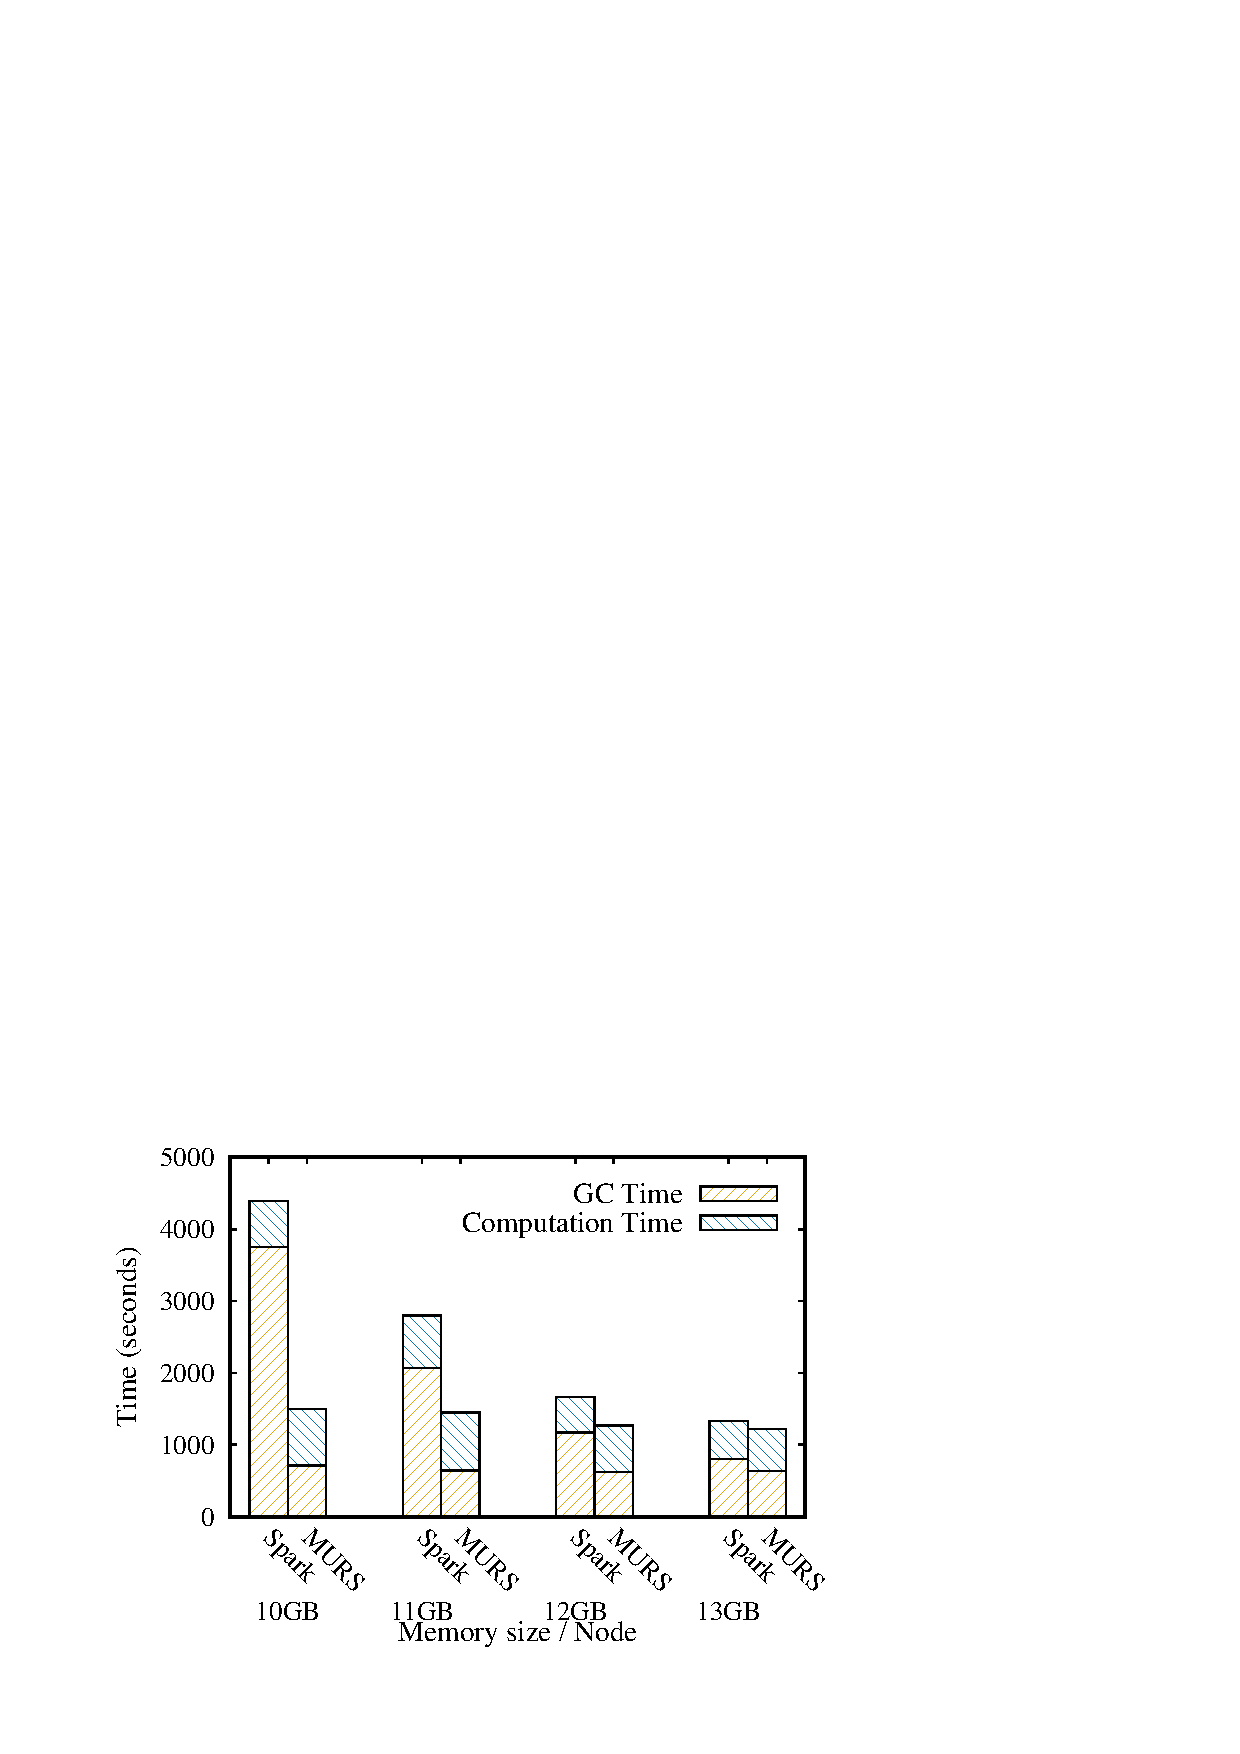
\includegraphics[width=0.23\textwidth]{sort-grep.pdf}}
%\hspace{-3ex}
\subfigure[AQ+SQ]{
\label{fig:subfig:wc-grep}
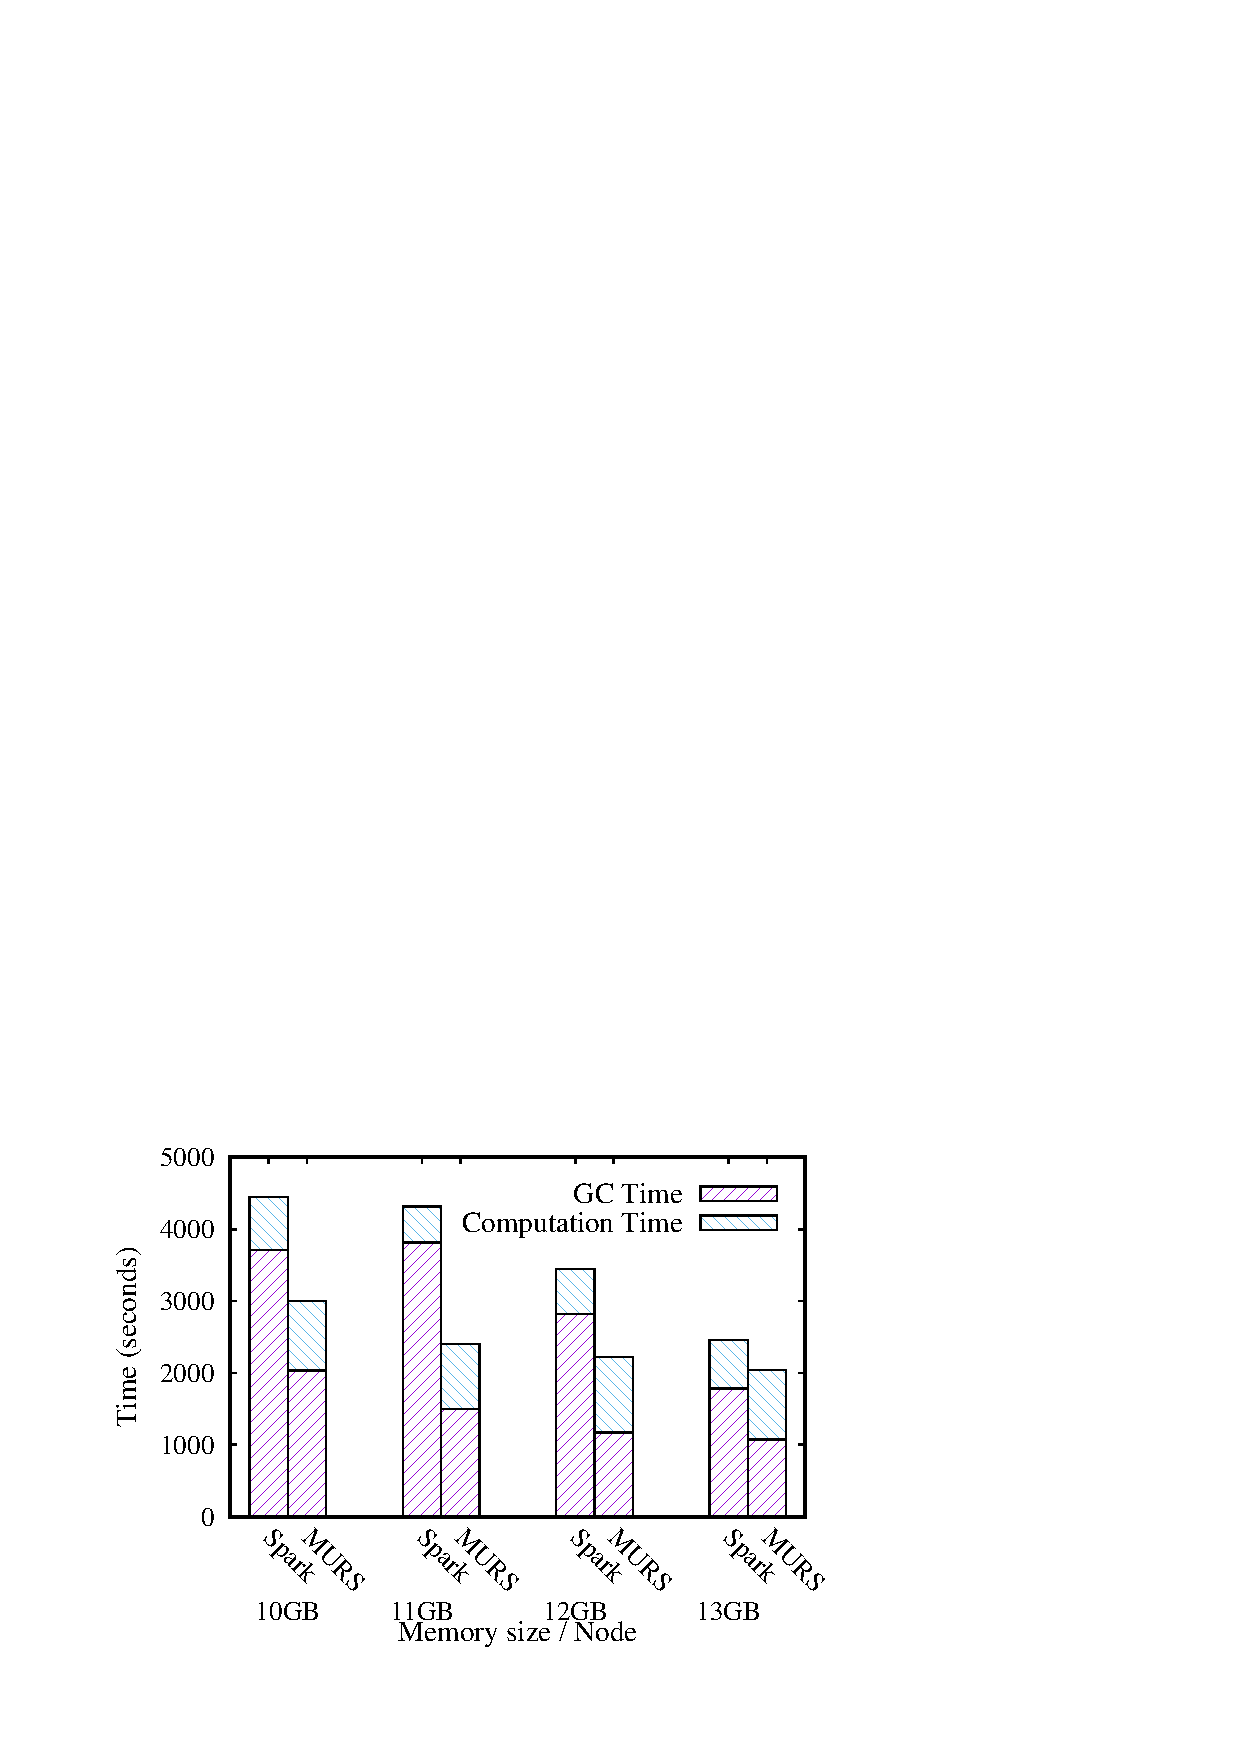
\includegraphics[width=0.23\textwidth]{wc-grep.pdf}}
%\hspace{-1.9ex}
\subfigure[Sort+AQ+SQ]{
\label{fig:subfig:sort-wc-grep}
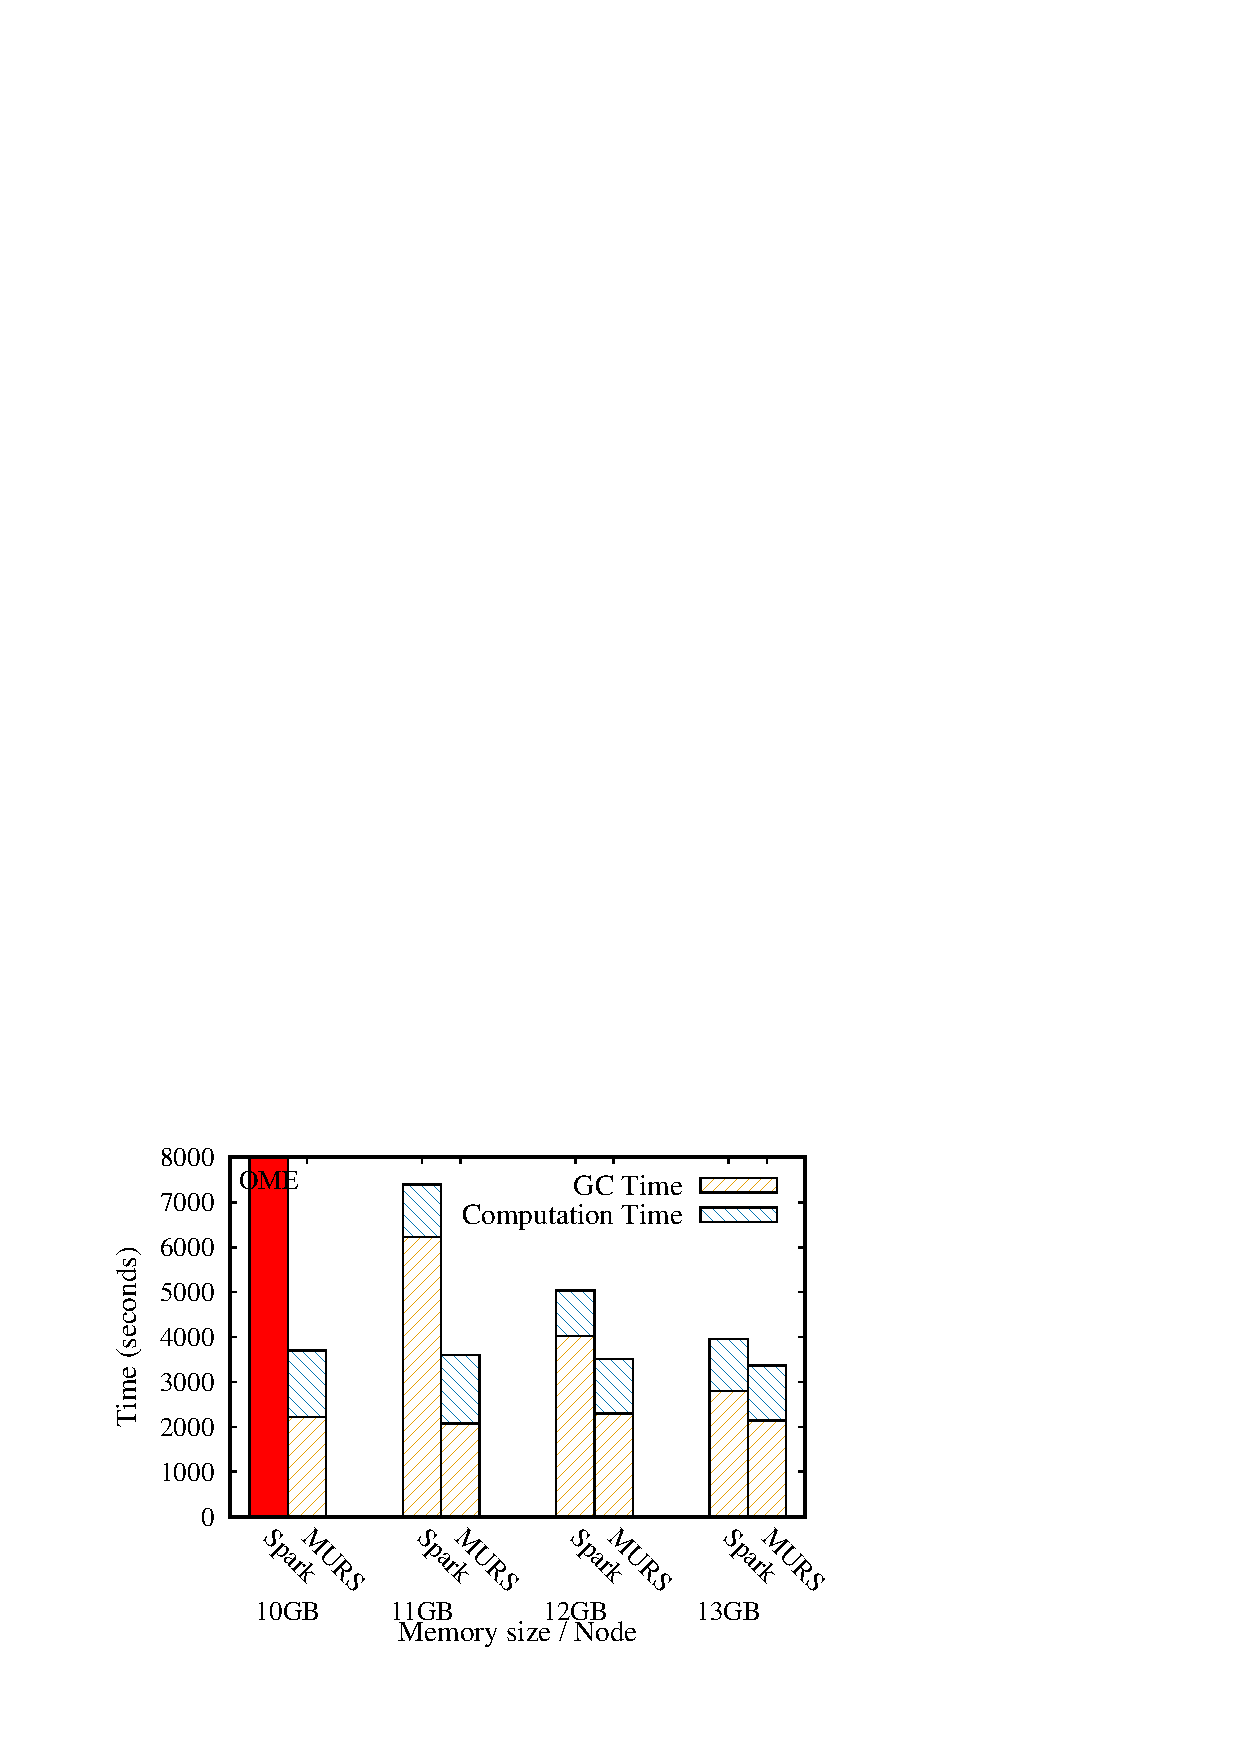
\includegraphics[width=0.23\textwidth]{sort-wc-grep.pdf}}
%\hspace{-1.9ex}
\subfigure[Active tasks]{
\label{fig:subfig:activetasks}
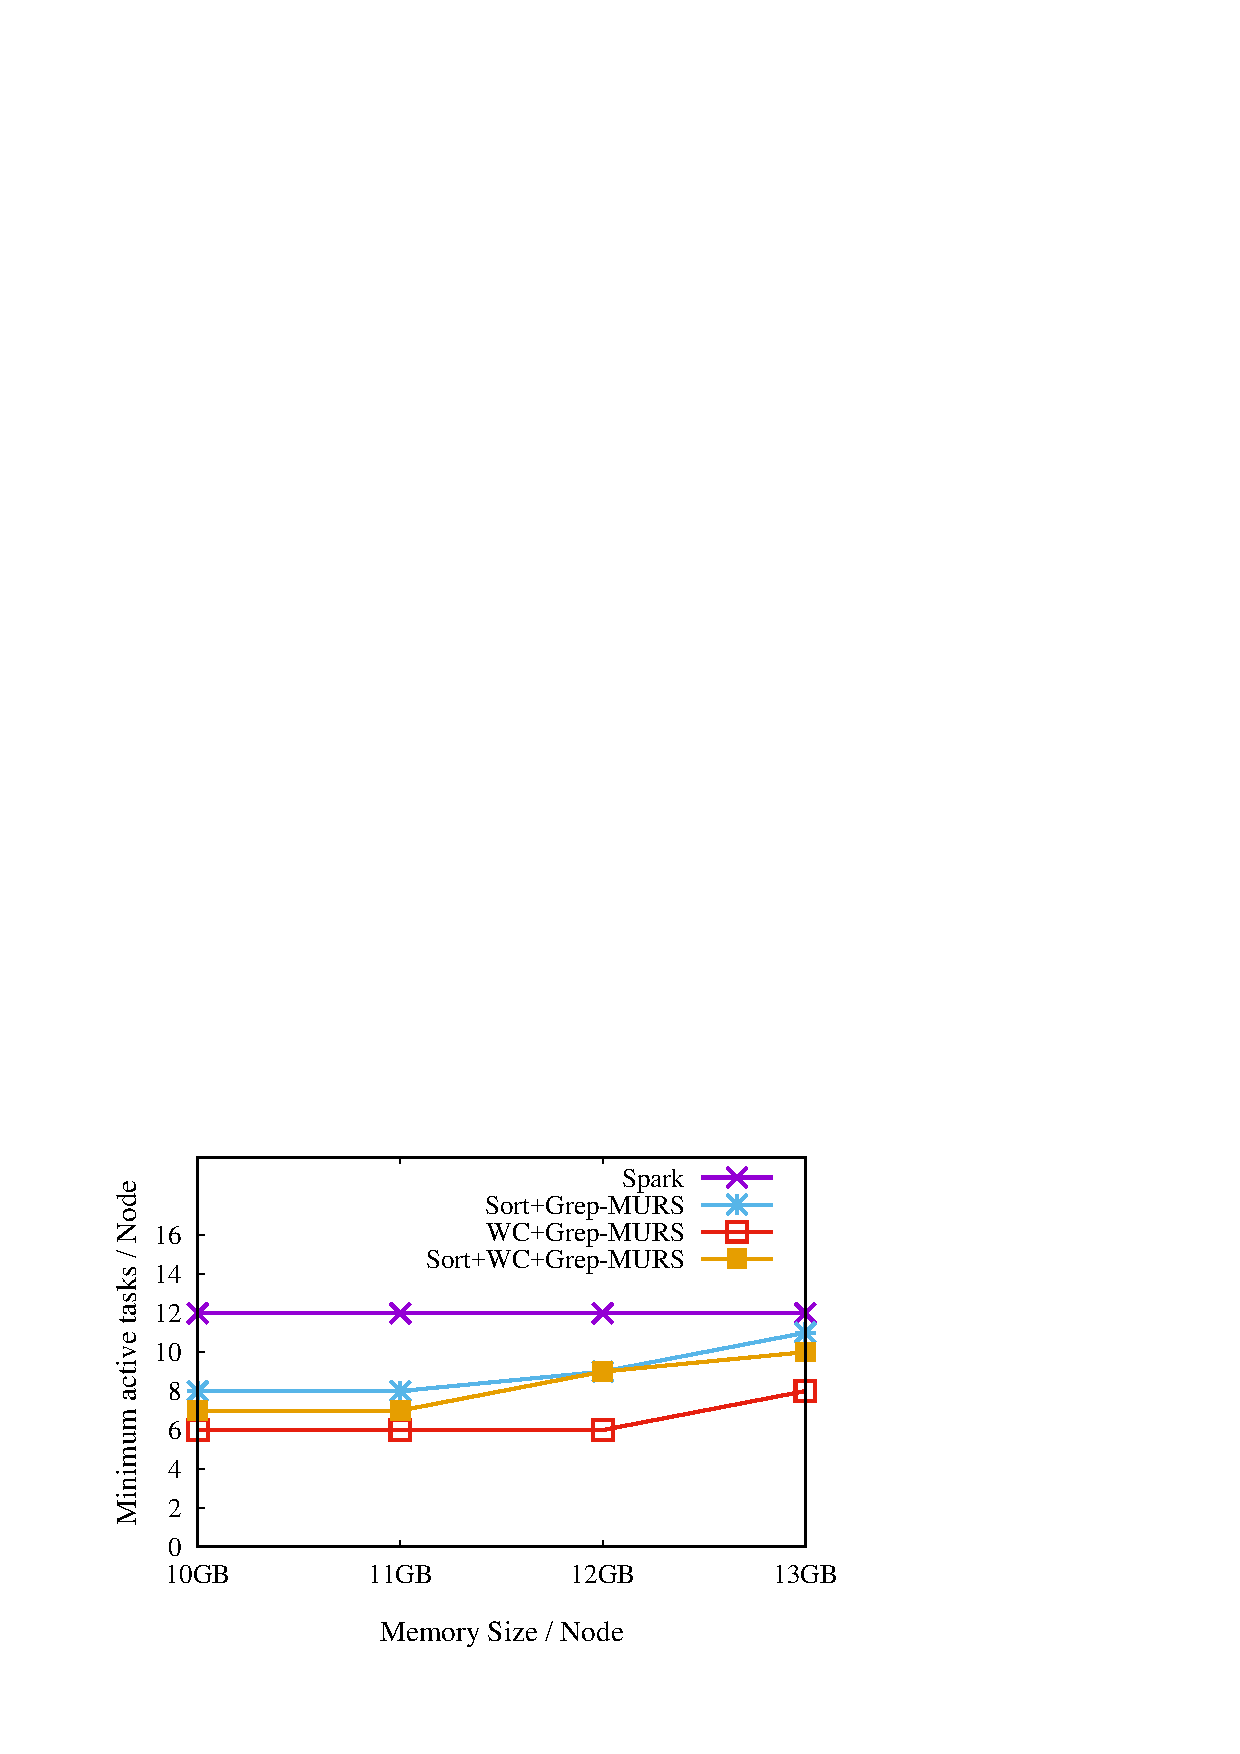
\includegraphics[width=0.23\textwidth]{active-task.pdf}}
\vspace*{-2mm}
\caption{Results of memory pressure without caching}
\vspace*{-4mm}
\label{fig:pressurewithoutcache}
\end{figure*}

When two applications are submitted to the server, MURS works better in Sort and SQ. Comparing Sort to AQ, the heavy memory pressure occurs in the different phase. The \textit{sort} operation is implemented in the \textit{read phase} of the tasks. Thus the tasks in the last stage of Sort suffer from the heavy memory pressure during their read phases. However, the \textit{reduce} operation in AQ is realized in the \textit{write phase} of the tasks. The heavy memory pressure is caused by the write phase of the tasks in the first stage. Moreover, massive temporary data objects are produced by the function API \textit{flatMap} before the write phase. They may be currently alive in the heap during the write phase in AQ. 
%Although the tasks in Sort belong to the linear memory usage model and the tasks in AQ are sub-linear
Thus, MURS suspends more tasks in AQ as the heap size in AQ is occupied by the temporary data objects, as shown in Figure~\ref{fig:subfig:activetasks}. These temporary data objects result in frequenter garbage collections. 
%We can see that suspension in MURS is determined not only by the memory usage models, but also by the current usage of the heap. 

When three applications are submitted, out-of-memory (OME) is thrown by the server. Although the live shuffle buffer in this case is smaller than the case with two applications, some other data objects occupy much heap space, such as the recording of living applications, the handler of disk writing, and the global configurations of Spark. Spark provides the spilling capability to overcome the shortage of memory. However, it cannot completely avoid the OME.

MURS mitigates the memory pressure in each application and we find that the performance decreases slowly as the heap size decreases. The result shows that the cost of garbage collection is stable. As MURS suspends the heavy tasks, the slow increase in execution time is due to the increase in computation time.  

\begin{comment}
\begin{figure}[!t]
\centering
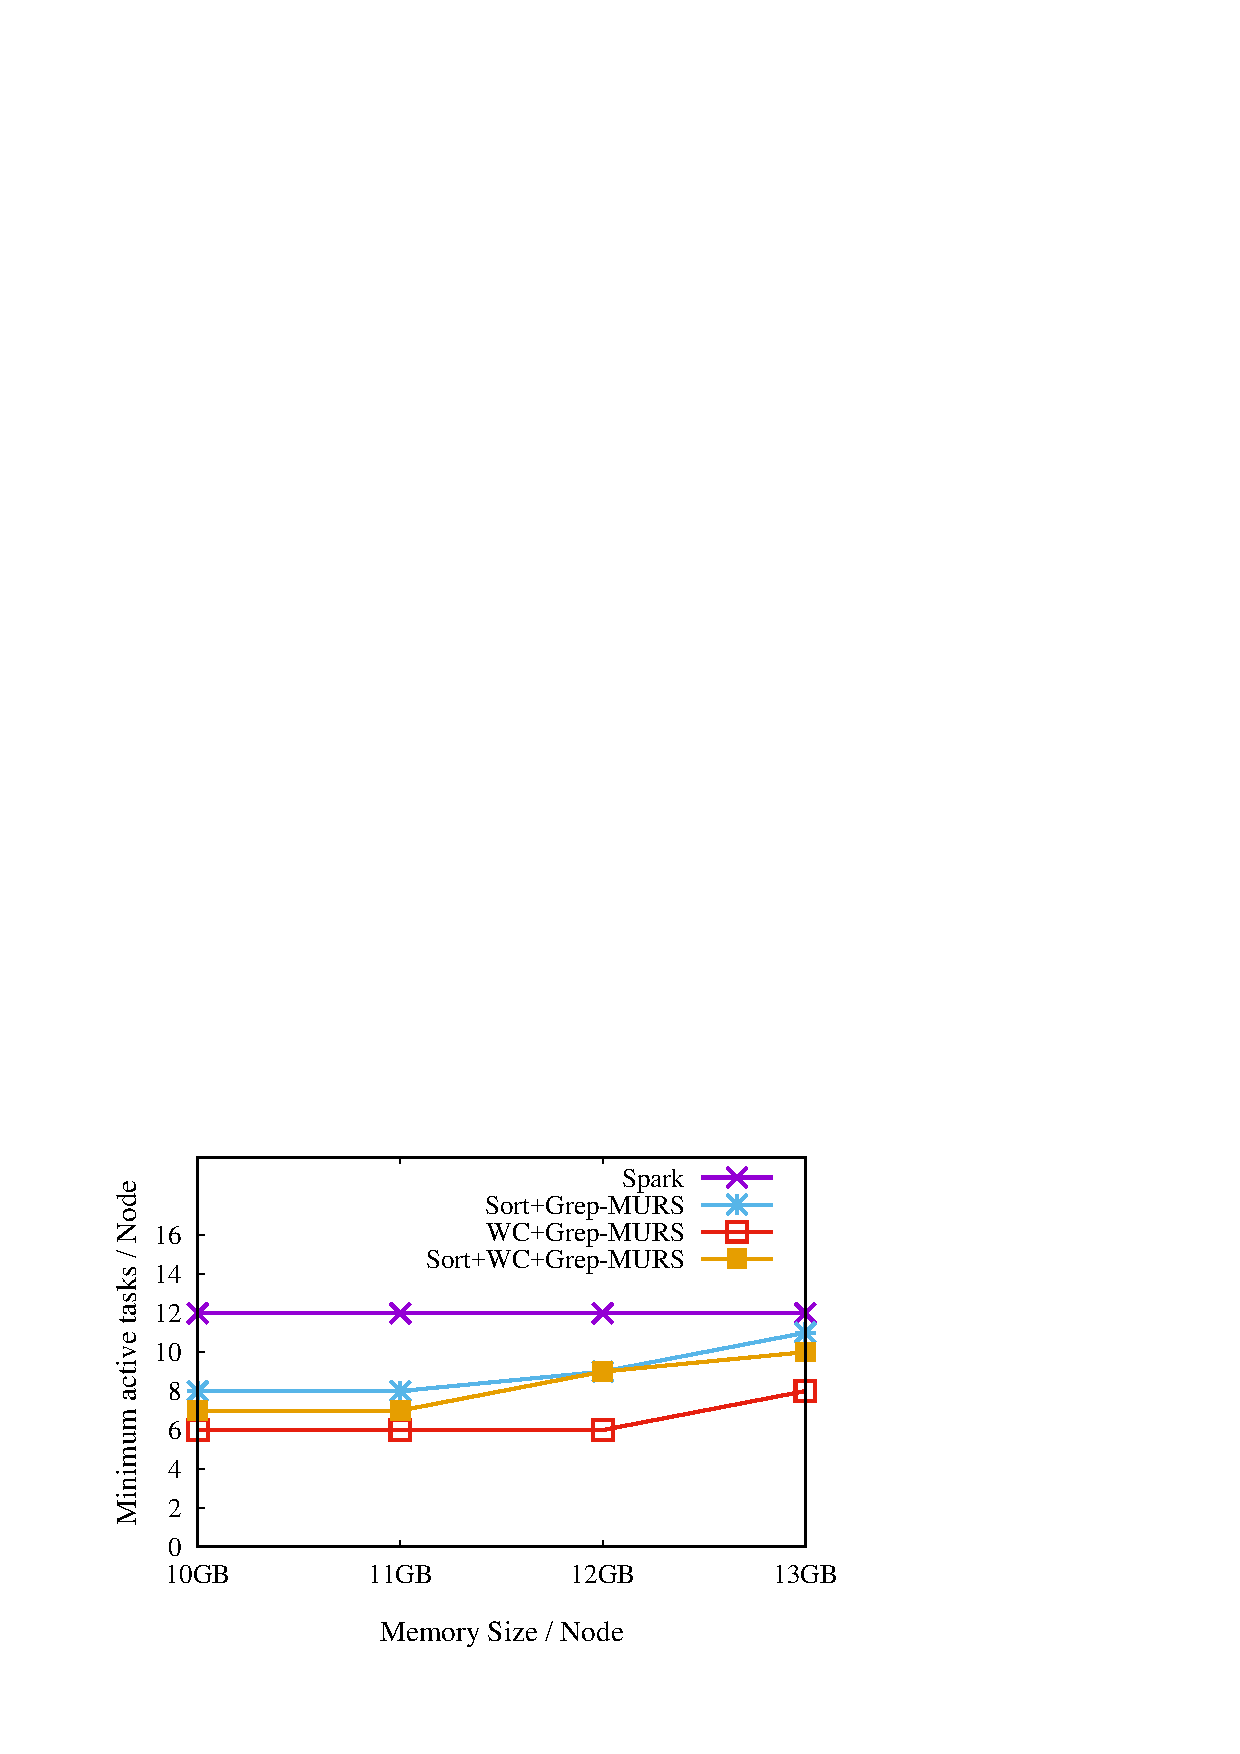
\includegraphics[width=0.35\textwidth]{active-task.pdf}
%\vspace{-2mm}
\caption{The minimum active tasks in each server}
%\vspace{-4mm}
\label{fig:active-task}
\end{figure}
\end{comment}

\subsection{Memory pressure with caching}

Some frameworks provide the caching mechanism for in-memory computation, such as Spark and Flink. Although the in-memory data caching speeds up the execution of a job, some works~\cite{bu:bloat, nguyen2015facade} show that it results in greater memory pressure because the cached data live as long as the job, especially when they are deployed as service-oriented systems. 
%Tracing these data is expensive. Also, the memory pressure means that there is less accessible memory space for the job execution.

PR and AQ are used as the experimental applications. PR is an iterative application. In the experiments, we run 5 iterations of the application. PR caches the intermediate data in memory after the first iteration. AQ is submitted at the second iteration. 
We adjust the heap size to show the performance of MURS, while the input dataset is 30GB, as shown in Figure~\ref{fig:cache-total}. When the heap size is less than 17GB, the service-oriented Spark throws the Out-of-Memory error (OME). MURS can provide the service when the heap size is reduced to 15GB. While they are both working, MURS improves the performance by up to 23.4\%, and the memory pressure is reduced by 65.4\%.

\begin{figure}[!t]
\centering
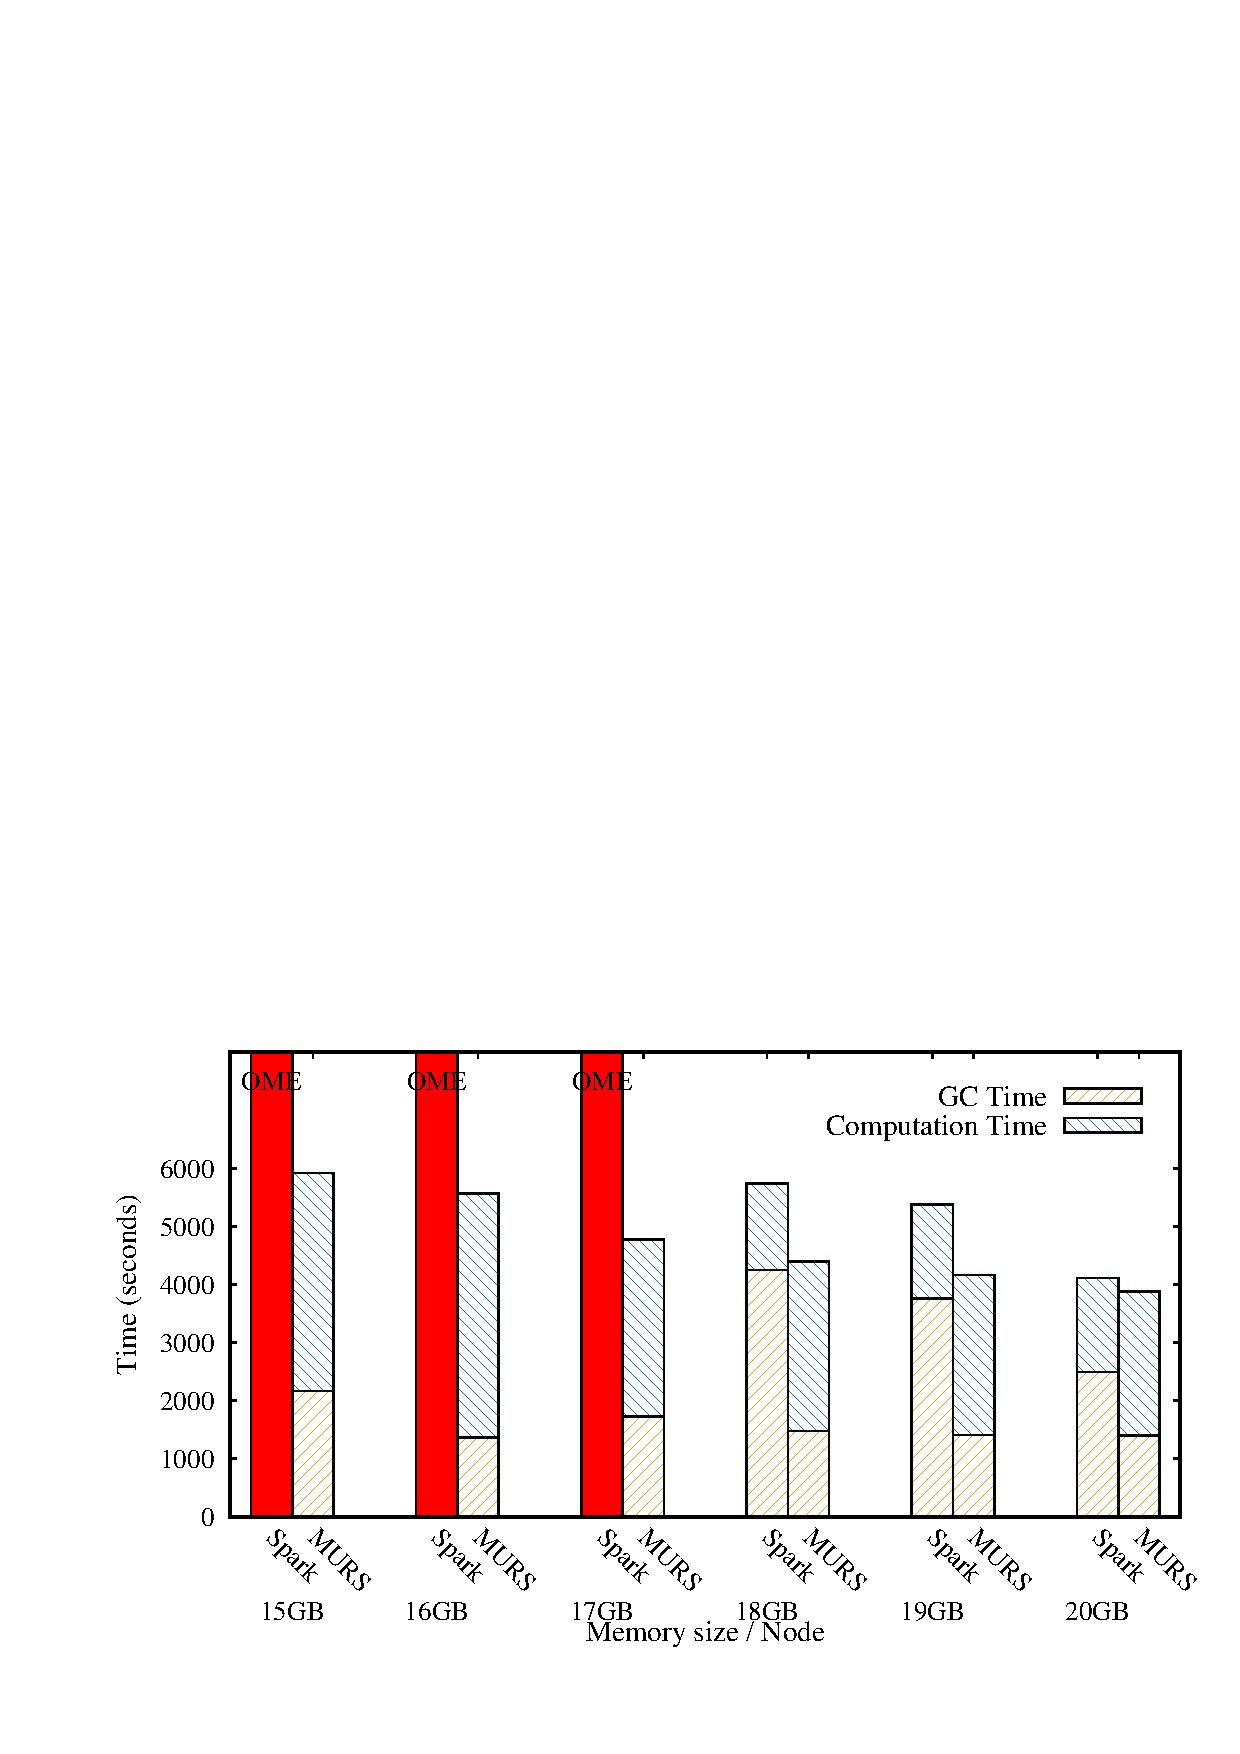
\includegraphics[width=0.4\textwidth]{cache-total.pdf}
\vspace{-2mm}
\caption{The Execution and GC Time of PR and AQ in Server}
\vspace{-4mm}
\label{fig:cache-total}
\end{figure}

Less heap size in each node means more memory pressure in the server. When the heap is exhausted, tasks will throw the OME. With the caching data in memory, The service-oriented Spark throws the OME as the heap size of each node is 17GB. However, MURS is able to mitigate the heavy memory pressure and still performs well when the heap size of each node is reduced to 15GB. MURS suspends heavy tasks and  thus the remaining light tasks can utilize more memory. Figure~\ref{fig:cache-peak} shows that the peak memory usage of all tasks in MURS is consistently larger than that in Spark. The number of active tasks in MURS is reduced to ensure there is the memory available for the running tasks. In other words, MURS has better scalability than the service-oriented Spark.

\begin{figure}[!t]
\centering
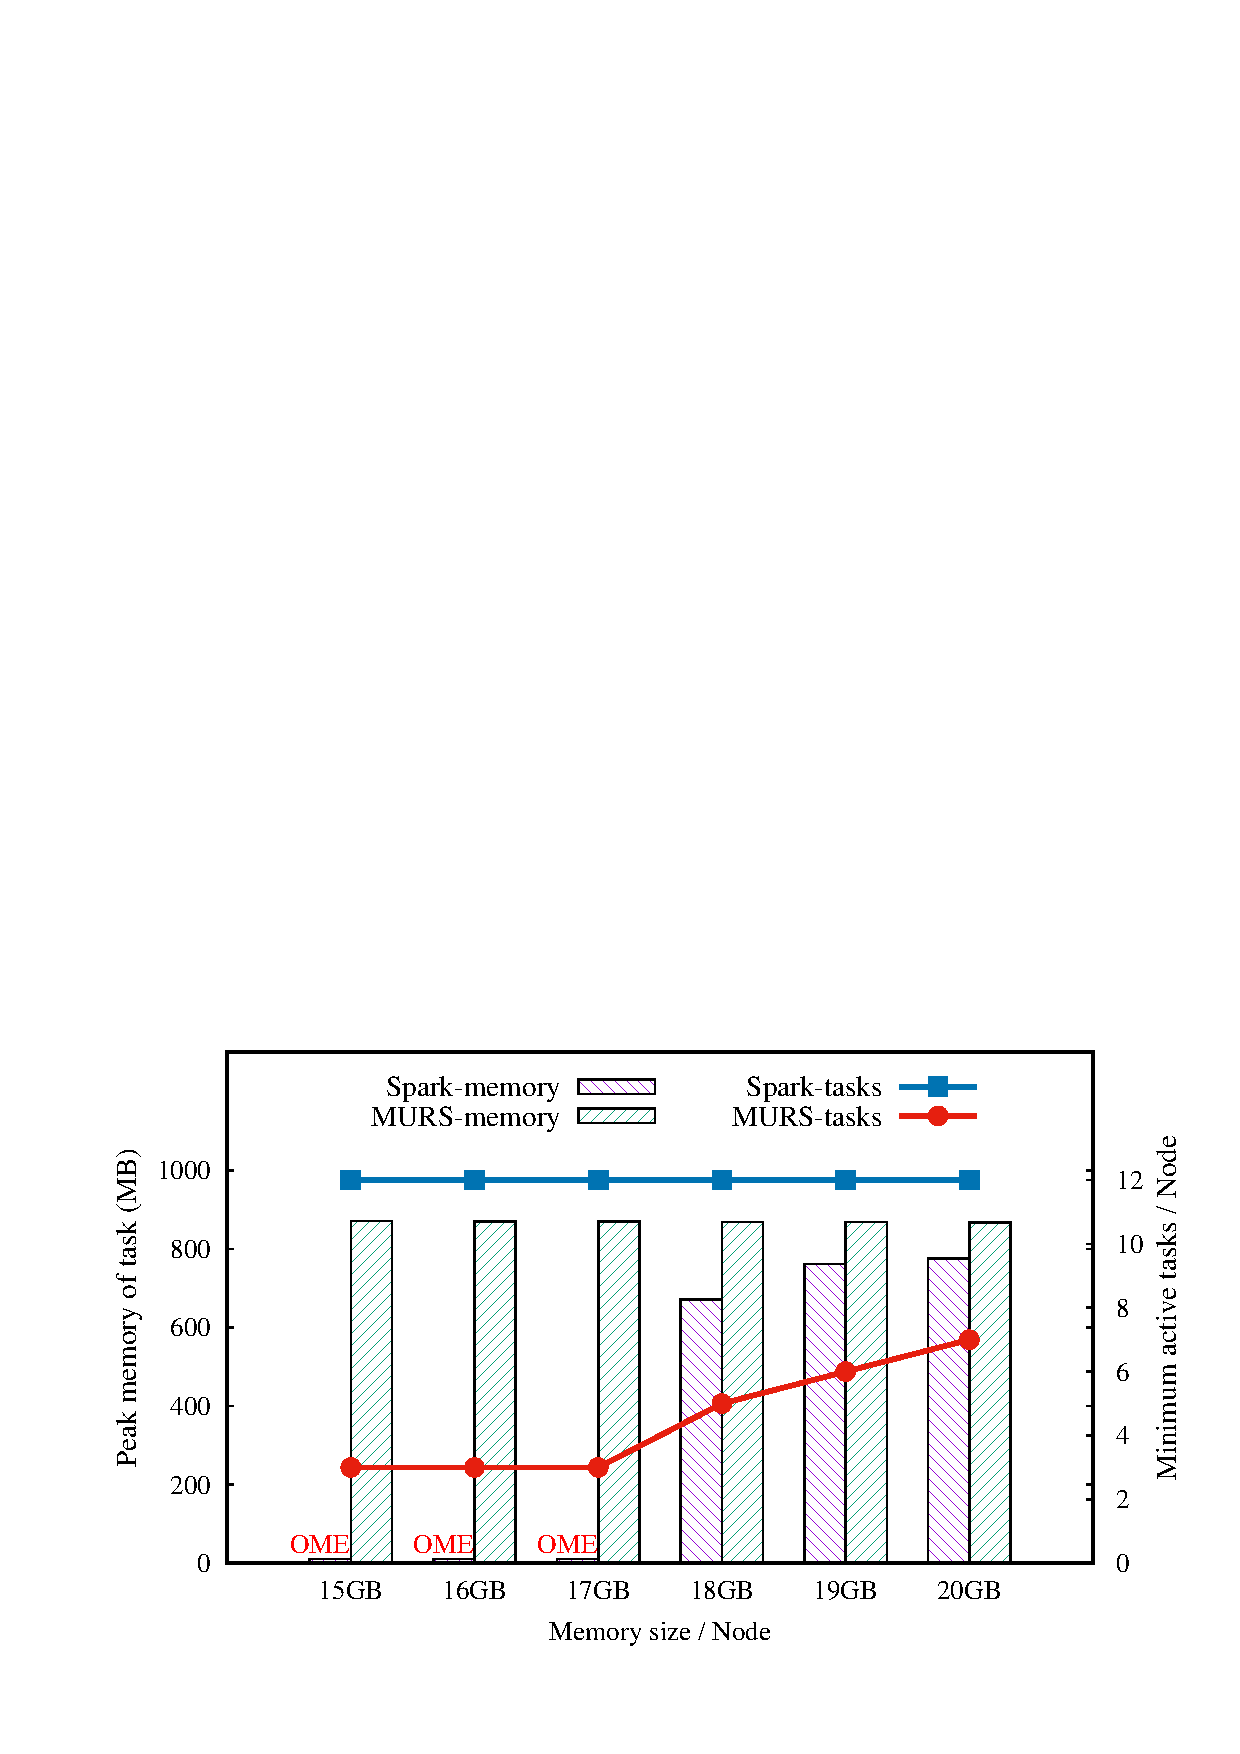
\includegraphics[width=0.4\textwidth]{cache-peak.pdf}
\vspace{-2mm}
\caption{The peak usage memory of tasks and minimum active tasks}
%\vspace{-2mm}
\label{fig:cache-peak}
\end{figure}

%\subsection{Potential starvation in MURS}

\begin{comment}
\textbf{Potential Starvation} The mitigation strategy of memory pressure delays the computation of suspended tasks. This may cause the starvation of the suspended tasks. MURS address this issue in the application level. 
%The settings of the experiment presented in this subsection are the same as those in the previous subsection. 
When PR and AQ are submitted to the server, t
%he tasks of PR have the same \textit{write phase} as the tasks of AQ, but contain more function APIs. Thus the tasks of PR are mostly classified as the heavy tasks. They will be suspended when the memory pressure is heavy. T
he execution time of each application is shown in Figure~\ref{fig:cache-prwc}. The result shows there is no starvation for PR. Benefiting from MURS, the performance of PR is improved by up to 24.4\%. The performance of AQ, which contains light tasks, also achieves a 29.8\% improvement. 

\begin{figure}[!t]
\centering
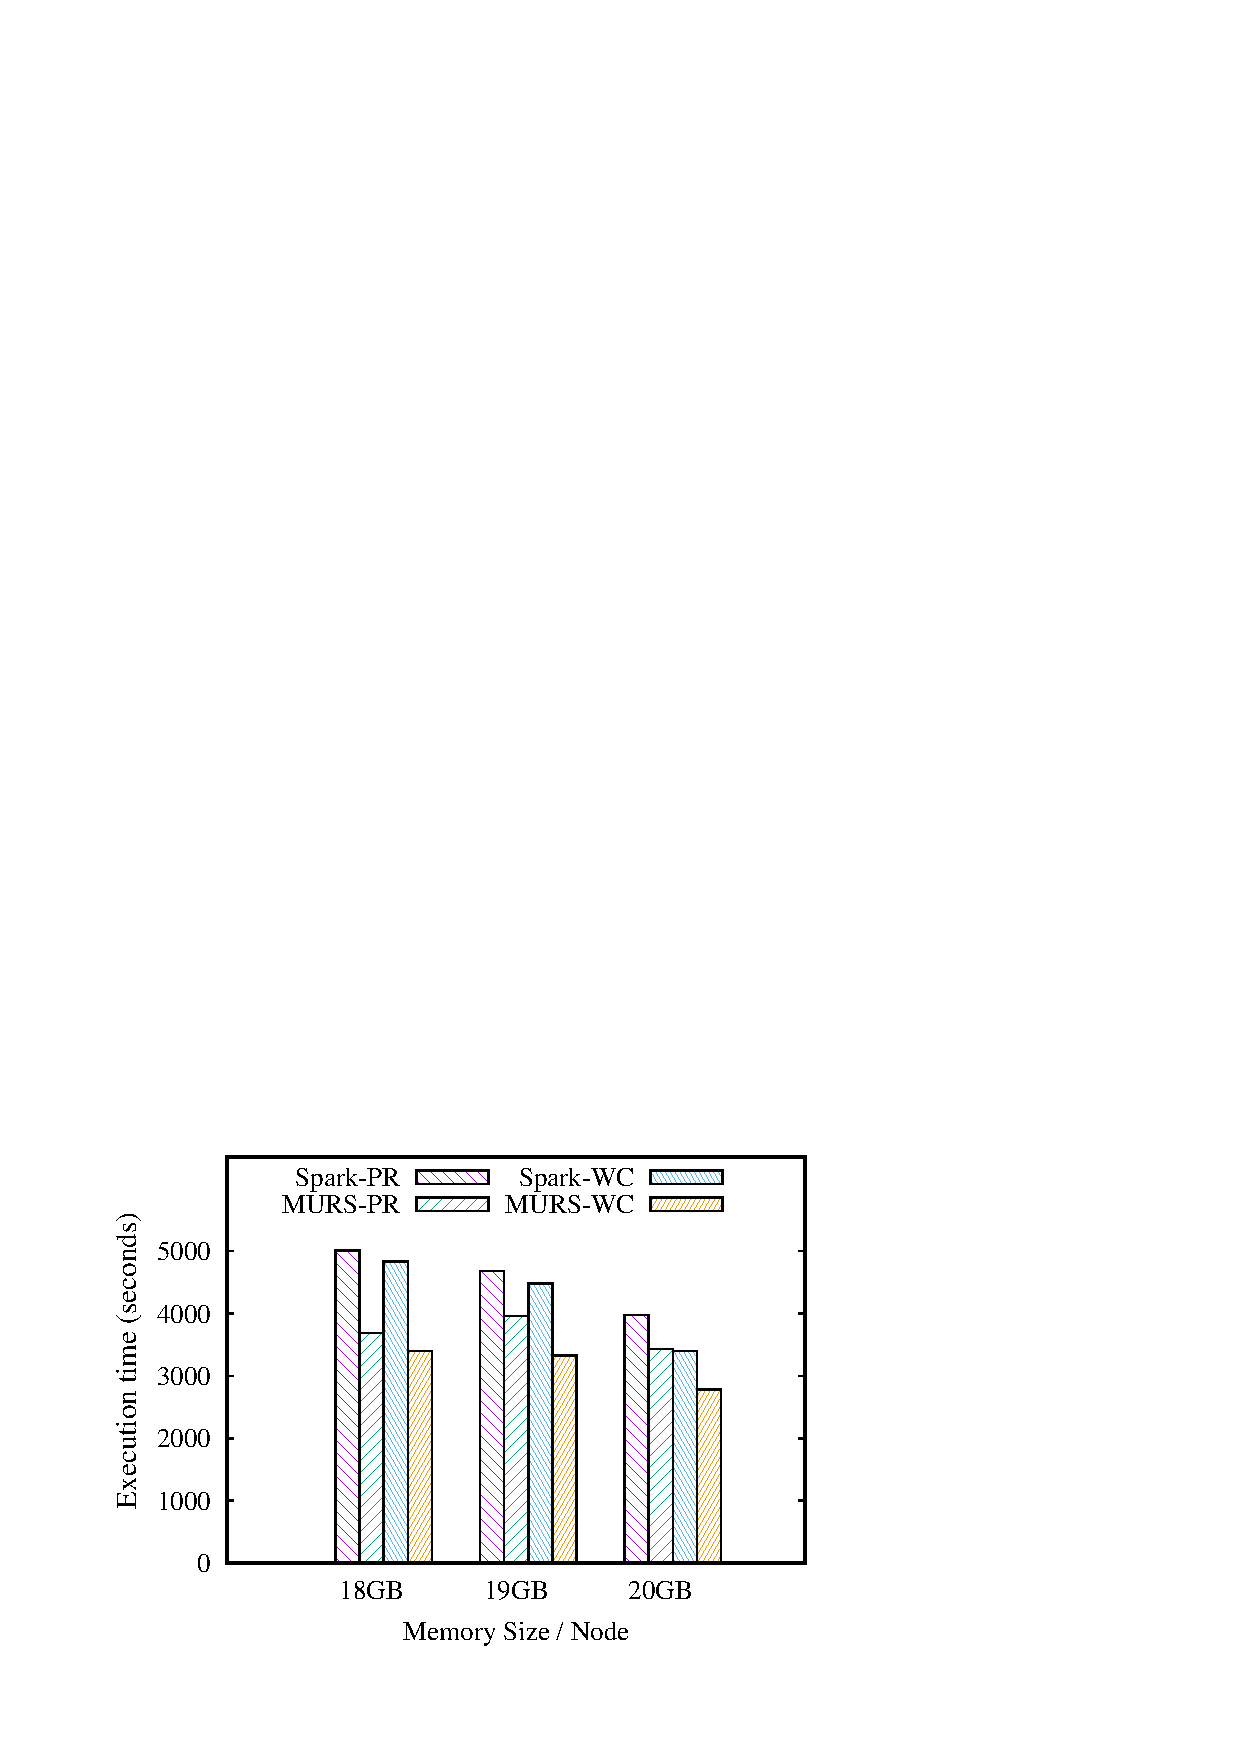
\includegraphics[width=0.3\textwidth]{cache-prwc.pdf}
\vspace{-2mm}
\caption{The execution time of each application}
\vspace{-2mm}
\label{fig:cache-prwc}
\end{figure}

MURS applies the FIFO algorithm when it resumes the suspended tasks. This avoids the long wait of these tasks. Otherwise, suspending these tasks is going to mitigate the memory pressure not only for the currently running light tasks, but also the heavy tasks running next. In the application level, the transient suspension and light memory pressure are actually the trade-off made by MURS. 

\end{comment}
%\subsection{Avoiding the spill}

\textbf{Avoiding the spill.} MURS sets the alarming threshold to avoid the spill when the memory pressure is heavy in the systems that allow the spill. 
%In the experiments presented in last subsection, we also measure the spilling tasks. MURS estimates the size of the required memory space for each task, and ensures that the running tasks can complete with the remaining memory space. 
%As the estimation is inaccurate to some extent, we find that fewer tasks will spill in MURS, as
Table~\ref{table:spill} shows the spill tasks in PR and AQ. There are no the spill tasks in AQ in MURS, while the spill tasks in PR decrease from 32\% to 2.5\%.
We notice that the error exists when avoiding the spill. The sampler in MURS counts two important metrics for a task: the percentage of the processed records in the total records, and the currently allocated memory space for this task. We can quickly obtain the required memory space based on these two metrics. When the memory pressure reaches the alarming threshold, we suspend a part of the running tasks and leave enough memory space for the remaining running tasks. As the estimate is based on sampling, the error exists in terms of the estimated size of the allocated memory space, especially when the value in some key-value pairs is a collection. 
%Different records have different sizes because the number of values inside a collection is different, such as \textit{groupByKey} in PR. Some hot keys may result in a substantial error. 
Thus, there are even fewer spilling tasks in MURS that the figures reported in the experiments.

\begin{table}[!t]
\small
\centering
\caption{Spill Tasks in MURS and Spark}
\begin{tabular}{ c | c | c | c | c | c }

\hline
\multirow{2}{*}{\textbf{App}} & \multirow{2}{*}{\textbf{Tasks}} & \multicolumn{2}{| c |}{\textbf{Spark}} & \multicolumn{2}{| c }{\textbf{MURS}} \\
\cline{3-6}
 & & spill & percent & spill & percent \\
\hline
AQ & 1000 & 91 & 9\% & 0 & 0  \\
\hline
PR & 1500 & 480 & 32\% & 37 & 2.5\% \\
\hline
%\multirow{2}{*}{MURS} & WC & 1000 & 0 & 0\% & - & - & -  \\
%\cline{2-8}
% & PR & 1500 & 37 & 2.5\% & 0 & 0 & 458 \\
%\hline

\hline
\end{tabular}
%\vspace{-2mm}
 
\vspace{-4mm}
\label{table:spill}
\end{table}
